\chapter{IRK: Eguzki-sistema.}


\section{Sarrera.}
  

Kapitulu honetan, eguzki-sistemaren ekuazio diferentzialei Kepler-en fluxuan oinarritutako aldagai aldaketa aplikatzea proposatuko dugu. \ref{chap:IRK-PF}~kapituluan puntu-finkoaren iterazioan oinarrituz eta \ref{chap:IRK-NEW}~kapituluan Newton sinplifikatuaren iterazioan oinarrituz, IRK inplementazioak garatu ditugu; eguzki-sistemaren problemaren integraziorako, bi inplementazioen artean, puntu-finkoarena eraginkorragoa dela baieztatu dugu. Ondorioz, puntu-finkoaren iterazioan oinarritutako IRK inplementazioa erabiliko dugu eta  ekuazio diferentzialetako aldagaiei eragingo diegun aldagai aldaketaren bidez, integrazio eraginkorra lortzea espero dugu.  

Aplikatzen dugun integrazio metodoa sinplektikoa eta simetrikoa da: neurri batean, Splitting metodoen baliokidea. Aldagai berriekiko ekuazio diferentzialak, magnitude txikiko balioak hartzen dituzte eta honek, hiru abantaila eragingo ditu. Lehenik, eguzki-sistemaren problemaren trunkatze errore nagusiena ezabatzen dugunez, urrats luzera handiagoak erabili ahal izango ditugu. Bigarrenik, batura konpensatuaren konputazioan, informazio gutxiago galduko dugu. Hirugarrenik, puntu-finkoaren iterazioek konbergentzia azkarra izango dute. 

Lehenengo, Kepler-en fluxuaren inplementazioa azalduko dugu. Bigarrenik, aldagai aldaketa definitu eta metodoa integratzeko zehaztapenak emango ditugu. Hirugarrenik, eguzki-sistemaren problemaren zenbakizko integrazioak egingo ditugu: inplementazio honen eta doitasun altuko beste metodo sinplektikoen (konposizio eta Splitting metodoak) eraginkortasunak, alderatuko ditugu.     

 

\section{Kepler-en fluxua.}
   
   
Kepler problema bi gorputzen problemaren kasu partikularra da eta  honako Hamiltondarra dagokio,
\begin{equation}
\label{eq: hamkepler}
H(q,p)=\frac{p^2}{2m}-\frac{\mu}{\|q\|},
\end{equation}
non $m$ eta $\mu$ konstanteen balioak, formulazioaren araberakoak diren.

Koordenatu sistema $q=q_2-q_1$ duen formulazioa aukeratzen badugu, konstanteen balioak hauek dira,  
\begin{equation*}
m=(1/m_1+1/m_2)^{-1},\ \ \mu=Gm_1m_2,
\end{equation*} 
%
eta ekuazio diferentzialak era honetan definitzen dira,
\begin{equation}
\label{eq:kode}
\dot{q}=p, \ \ \dot{p}= - \frac{k \ q}{\|q\|^3} ,
\end{equation}
non $k= \mu / m$ eta  $q,p \in \mathbb{R}^3$ diren.

Kepler problemaren soluzio zehatza kalkula daiteke: une bateko kokapen eta abiadurak emanik, $\Delta t$ denbora tarte bat igarotakoan (positiboa ala negatiboa), kokapen eta abiadura zehatzak konputatu daitezke. Eguzki-sistemaren integrazioetarako, Kepler problema doitasun handian eta era eraginkorrean kalkulatzea, funtsezkoa da. Kepler problemaren erreferentziazko inplementazioak, Danby \cite{Danby1992} eta J.Wisdom-enak  \cite{Wisdom2015} ditugu. 

Kepler-en fluxua, era honetan kalkulatzen da. Lehenik, koordenatu cartesiarretatik ($q,p\in \mathbb{R}^3$), koordenatu eliptikoetara $(a,e,i,\Omega,E)$ itzulpena egingo dugu. Koordenatu eliptikoetan, $E$ (\emph{eccentric anomaly}) aldagaia izan ezik, beste aldagaiak konstante mantentzen dira: beraz, $E_0$ balioa emanda, $\Delta t$ denbora tartea aurrera egin eta $E_1$ balio berria kalkulatuko dugu. Azkenik, koordenatu eliptikoetatik koordenatu cartesiarretara itzulpena eginez, kokapen eta abiadura berriak eskuratuko ditugu. 

\begin{equation*}
(q_0,v_0) \in \mathbb{R}^6 \ \ \ \longrightarrow \ \ \  (a,e,i,\Omega,E_0) \in \mathbb{R}^6 
\end{equation*}
\begin{equation*}
\quad \quad \quad \quad \quad \quad \quad \quad \downarrow \Delta t
\end{equation*}
\begin{equation*}
(q_1,v_1) \in \mathbb{R}^6 \ \ \ \longleftarrow \ \ \  (a,e,i,\Omega,E_1) \in \mathbb{R}^6 
\end{equation*}

Gorputz baten orbita Kepleriarra hiru motakoa izan daiteke: $H(q_0,p_0)<0$ denean orbita eliptikoa da, $H(q_0,p_0)>0$ orbita hiperbolikoa eta $H(q_0,p_0)=0$ orbita  parabolikoa. Kepler fluxuaren C inplementazioa, orbita eliptikoetarako garatu dugu eta zehaztasunak, \ref{erans:B1} eranskinean eman ditugu. (\ref{eq:kode}) problemari dagokion fluxua, era honetan defini daiteke,
\begin{align*}
\varphi_{\Delta t}^k:&  \quad \mathbb{R}^{6} \quad  \longrightarrow \quad \mathbb{R}^6,  \\
&  \quad u_0 \ \  \rightsquigarrow \ \ u_1. 
\end{align*} 
non $u=(q,v) \in \mathbb{R}^6$  den.

\section{Kepler Perturbatuaren problema.}

Kepler problemaren Hamiltondarra perturbatzen badugu, ezingo dugu aurreko atalean erabili dugun fluxua erabili problema ebazteko. Kasu honetan Hamiltondarra  bi zatitan banatuta egongo da;
\begin{align}
\begin{split}
\label{eq: hamkeplerpert}
&H(q,p,t)=H_K(q,p)+H_I(q,p,t)
\end{split}
\end{align} 
non $H_K$ mugimendu Kepleriarrari dagokion Hamiltondarraren aldea den, hau da, (\ref{eq: hamkepler}) ekuazioko eskuin aldea, eta $H_I$ perturbazioei dagokien Hamiltondarraren aldea den.

Problema berri honetan aldagai aldaketa bat egingo dugu, aldaketaren helburua da Keplerren fluxua erabili ahal izatea problemaren ebazpenean. 

\subsection*{Aldagai aldaketa.}

%Kontutan hartuko ditugun sistemak Hamiltondarrak dira, $H: \mathbb{R} \times \mathbb{R}^{2d} \longrightarrow \mathbb{R}$, gainera, Hamiltondarra bi zatitan bana dakieken sistemak hartuko ditugu kontuan:

(\ref{eq: hamkeplerpert}) problemari dagozkion ekuazioetan, Keplerren fluxuan oinarritutako aldagai aldaketa bat egingo dugu, baina horretarako notazioa finkatuko dugu: jatorrizko aldagaiak $u=(q,p) \in \mathbb{R}^{2d}$ izango dira eta aldagai berriak $U=(Q,P) \in \mathbb{R}^{2d}$ letra larriz adieraziko ditugu. Jatorrizko aldagaien bidez adierazitako problema, alegia, ebatzi beharreko hasierako baliodun problema, honakoa da:

\begin{align}
\begin{split}
\label{eq: HamEDA}
&\frac{du}{dt} = k(u) + g(u,t),\ \ \ u(0) = u_0
\end{split}
\end{align} 
non $k(u)$ alde Kepleriarrari dagokion eta $g(u,t)$ perturbazioari. 
Problema horretan honako aldagai aldaketa egingo dugu, kontuan izan urrats bakoitzean egingo dugula aldagai aldaketa, hau da $j=0, 1, 2 \ldots$ indizeak $j$. urratsean aplikatu beharreko aldaketa adierazten du:

\begin{align}
\begin{split}
\label{eq: uUaldaketa}
&u(t) = \varphi_{t-(j+\frac{1}{2})h}^k\left(U_j^{j+\frac{1}{2}}(t)\right)
\end{split}
\end{align} 
$\varphi_{\Delta t}^k$ fluxua $\Delta t>0$ eta $\Delta t <0$ balioentzat definitzen da, eta  $u= \varphi_{-t}(\varphi_{t}(u))$ betetzen dela kontutan hartuz honako alderantzizko aldaketa ere egin dezakegu:
\begin{align}
\begin{split}
\label{eq: Uualdaketa}
U^{j+\frac{1}{2}}(t) = \varphi^k_{-t+(j+\frac{1}{2})h} \left( u(t) \right)
\end{split}
\end{align} 

Aldaketa hauekin asmoa da $i+1$ urratsa emateko $u_i \approx u(hi)$ zenbakizko soluzioan oinarrituz, aldagai aldaketaren bidez $U_i^{i+\frac{1}{2}}=\varphi^k_{\frac{h}{2}}(u_i)$ lortu, hau da, fluxuan $\frac{h}{2}$ aurrera egin aldagai berriak lortzeko, aldagai berri hauetan ebatzi jatorrizko problemaren urrats bati dagokion zenbakizko soluzioa (ikusiko dugun bezala, aldagai berrietan alde Kepleriarrari dagokion espresioak ez du eraginik eta, azken finean perturbazioari dagokion aldaketa da hemen kalkulatuko dena) eta azkenik, aldagai berri hauen balio berriak jatorrizko aldagaietara itzuli behar dira, baina $i+1$ urratsari dagozkion unera pasa behar dira aldagaiak, hau da, fluxuan aurrera $\frac{h}{2}$ egin behar da. Atzera egingo bagenu urratsaren hasierako balioei perturbazioak zein aldaketa eragiten dien kalkulatuko baikenuke, baina guk urratsaren bukaerako balioak nahi ditugu. Laburbilduz:


\begin{align*}
   &   \quad U_0^{\frac{1}{2}} \quad \quad \quad \quad \Longrightarrow  & U_1^{\frac{1}{2}}&  &\\
  & \nearrow \varphi_{\frac{h}{2}}(u_0) &            & \searrow \varphi_{\frac{h}{2}}(U_1)& \\
u_0 &                  &    &\quad \quad \quad  u_1
\end{align*}

Aldagai aldaketak fluxuan aurrera egiten du urratsaren luzeraren erdia. Hori horrela egiteak badu arrazoi bat: urratsa bere osotasunean simetrikoa da. Aurrera $h$ luzerako urratsa ematea $-h$ luzerako urratsa ematearekin desegiten baita. 

%\begin{figure}[h!]
%\centering
%\subfloat[Aldagai aldaketa.]{
%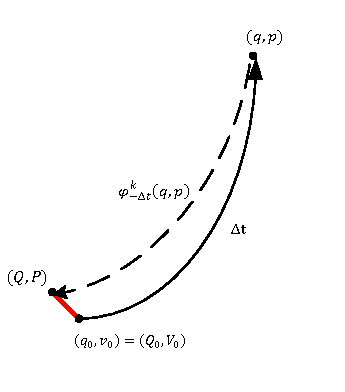
\includegraphics[width=.400\textwidth]{Aldagaialdaketa1}
%}
%\subfloat[Aldagai berrien integrazioa.]{
%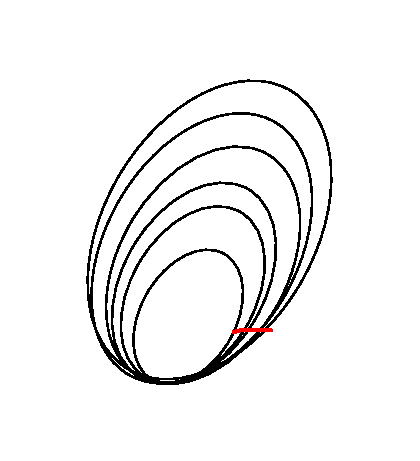
\includegraphics[width=.400\textwidth]{Aldagaialdaketa2}
%}
%\caption[Atalen hasieraketa.]
%        {\small (a)irudian, aldagai aldaketa irudikatu dugu eta (b) irudian, perturbatutako gorputza baten orbitaren integrazioak erakutsi ditugu. Bi irudietan, $(Q,P)$ balioen aldaketa txikiak gorriz nabarmendu ditugu          
%        }
%\label{fig:Aldg}
%\end{figure}   

\subsection*{Aldagai berrietan ekuazio diferentzialak.}

(\ref{eq: uUaldaketa}) aldagai aldaketa abiapuntutzat hartuz, aldagai berriei dagozkien ekuazio diferentzialak lortu behar ditugu. Horrela, problemaren integrazioa aldagai berrien arabera egin ahal izango dugu. Irakur erraztasunagatik (\ref{eq: uUaldaketa}) ekuazioko $\varphi(U)$ indizerik gabe idatziko dugu, eta $\dot{U}$ri dagozkion ekuazioak lortze aldera bi aldeak $t$ aldagaiarekiko deribatuko ditugu:  
\begin{align}
\begin{split}
&\frac{d}{dt}u = \frac{d}{dt}\left(\varphi(U)\right),
\end{split}
\end{align}
Eskuin aldeari katearen erregla aplikatuz, 
\begin{align}
\begin{split}
&\dot{u} = \dot{\varphi}(U) + \varphi'(U) \frac{d}{dt}U.
\end{split}
\end{align}
$\varphi$ Kepler problemaren fluxua da, hau da, $\dot{u} = k(u)$ problemaren fluxua da, eta fluxuaren definizioz $\dot{\varphi}(U) = k(\varphi(U))$ da. Aldaketa horrekin,  eta (\ref{eq: HamEDA}) ekuazioarekin berdinduz,
\begin{align}
\begin{split}
&k(u) + g(u,t) = k(u) + \varphi'(U) \dot{U}.
\end{split}
\end{align}
Bi aldeetan $k(u)$  kenduz, $U$ aldagaiekiko ebatzi beharreko ekuazio diferentziala lortuko dugu:
\begin{align}
\begin{split}
\label{eq:hamEDAU}
&\dot{U} = \left(\varphi'(U)\right)^{-1} g(u,t).
\end{split}
\end{align}
Alderantzizko matrizeak kalkulatu beharrik gabe idatz ditzakegu (\ref{eq:hamEDAU}) ekuazioak. Horretarako $\varphi$ fluxuaren izaera sinplektikoa erabiliko dugu, hau da, $(\varphi')^tJ\varphi'= J$ propietatea betetzen du fluxuak, ondorioz,
%
\begin{align}
\begin{split}
\label{eq:hamEDAU2}
&\dot{U} = J^{-1}(\varphi')^{t}(U)J g(u,t).
\end{split}
\end{align}
(\ref{eq:hamEDAU2}) ekuazioak $\varphi'(U)$ kalkulatzea eskatzen du, eta horretarako deribazio automatikoko teknikak erabil ditzakegu.


\paragraph*{Algoritmoa.}
$U$ aldagaietan oinarritutako ekuazio diferentzialen integraziorako (\ref{eq:hamEDAU2}) espresioaren konputazioa hiru urratsetan egingo dugu:
\begin{enumerate}
\item $\{u,aux\} \leftarrow KeplerFlowGen (t,U,mu)$.

Kepler-en fluxua $u= \varphi_t(U)$ aplikatuko dugu eta fluxuaren kalkulutarako erabilitako tarteko balioak, ~$aux\in \mathbb{R}^{16}$ aldagaian itzuliko ditugu. 

\item $g \leftarrow g(u,t)$.

Jatorrizko problemako ekuazio diferentzialetan perturbazioei dagokien espresioa kalkulatuko dugu.

\item $KeplerFlowGFcnaux(aux,U,t,g)$.

Urrats honetan $\varphi'_t()$ kalkulatu behar da. Deribazio automatikoaren tekniken bidez, Kepler fluxuaren $U$ aldagaiekiko deribatuaren konputazio eraginkorra definitu dugu. 

Hirugarren urratsak (\ref{eq:hamEDAU2}) espresioa konputatzeko behar dugun azken zatia kalkulatzen du, beraz, bere emaitza $\dot{U}$ren konputazioa izango da: 
\begin{align*}
\dot{U}&\leftarrow KeplerFlowGFcnaux(aux,U,t,g) = ( \varphi'(U))^{-1} \ g.
\end{align*}

\end{enumerate} 



\section{Alde Kepleriar bat baino gehiagoko sistemak.}

Alde Kepleriar bat baino gehiago dituzten problemetan ere Kepler perturbatuan egindako aldagai aldaketa egin dezakegu. Hainbat gorputzeko sisteman gorputz bakoitzari eragingo diogu aldagai aldaketa, bakoitzak bere fluxu Kepleriar perturbatua izango du, eta horretan oinarrituz egingo diogu aldaketa. Problemaren alde Kepleriarren kopurua $k$ bada, era honetako ekuazio diferentzialak ditugu,
\begin{equation}
\label{eq: n-pertEDA}
\frac{d}{dt}\left(\begin{array}{c}
                u  \\
                w  \\
\end{array}\right)=
\left(\begin{array}{c}
                \dot{u}_1  \\
                \dot{u}_2  \\
                \vdots \\
                \dot{u}_k    \\
                \dot{w}      \\
\end{array}\right)=
\left(\begin{array}{c}
                k(u_1)  \\
                k(u_2)  \\
                \vdots \\
                k(u_k)  \\
                0      \\
\end{array}\right)+
\left(\begin{array}{c}
      g_1(u_1, u_2\dots, u_k,w,t) \\
      g_2(u_1, u_2\dots, u_k,w,t) \\
                \vdots \\
      g_k(u_1, u_2\dots, u_k,w,t)\\
      g_{k+1}(u_1, u_2\dots, u_k,w,t)
\end{array}\right)
\end{equation} 

Gorputz bakoitzari dagokion aldagai aldaketa bere fluxu Kepleriarraren araberakoa da,
\begin{align}
\label{eq:aldfl2}
\begin{split}
u_j&= \varphi_t^{\mu_j}(U_j), \ \ \ j=1,\dots,k.
\end{split}
\end{align}
Bi aldeak $t$ aldagaiarekiko deribatuz eta katearen erregela aplikatuz,
\begin{equation*}
\left(\begin{array}{c}
                \dot{u}_1  \\
                \dot{u}_2  \\
                \vdots \\
                \dot{u}_k    \\
                \dot{w}      \\
\end{array}\right)=
\left(\begin{array}{c}
                \dot{\varphi}^{\mu_1}(U_1)  \\
                \dot{\varphi}^{\mu_2}(U_2)   \\
                \vdots \\
                \dot{\varphi}^{\mu_k}(U_k)   \\
                0      \\
\end{array}\right)+
\left(\begin{array}{c}
      (\varphi^{\mu_1})'(U_1) \frac{d}{dt}U_1 \\
      (\varphi^{\mu_2})'(U_2) \frac{d}{dt}U_2 \\
                \vdots \\
      (\varphi^{\mu_k})'(U_k) \frac{d}{dt}U_k\\
      g_{k+1}(u_1, u_2\dots, u_k,w,t)
\end{array}\right),
\end{equation*}
ekuazioetan fluxuen propietate eta definizioak erabiliz,
\begin{equation*}
\left(\begin{array}{c}
                \dot{u}_1  \\
                \dot{u}_2  \\
                \vdots \\
                \dot{u}_k    \\
                \dot{w}      \\
\end{array}\right)=
\left(\begin{array}{c}
                k(u_1)  \\
                k(u_2)   \\
                \vdots \\
                k(u_k))   \\
                0      \\
\end{array}\right)+
\left(\begin{array}{c}
      (\varphi^{\mu_1})'(U_1) \dot{U}_1 \\
      (\varphi^{\mu_2})'(U_2) \dot{U}_2 \\
                \vdots \\
      (\varphi^{\mu_k})'(U_k) \dot{U}_k\\
      g_{k+1}(u_1, u_2\dots, u_k,w,t)
\end{array}\right),
\end{equation*}
eta, azkenik, (\ref{eq: n-pertEDA}) ekuazioarekin berdinduz eta sinplifikatuz,
\begin{equation*}
\left(\begin{array}{c}
                \dot{U}_1  \\
                \dot{U}_2  \\
                \vdots \\
                \dot{U}_k    \\
                \dot{w}      \\
\end{array}\right)=
\left(\begin{array}{c}
      \left((\varphi^{\mu_1})'(U_1)\right)^{-1} g_1 \\
      \left((\varphi^{\mu_2})'(U_2)\right)^{-1} g_2 \\
                \vdots \\
     \left((\varphi^{\mu_k})'(U_k)\right)^{-1} g_k\\
      g_{k+1}
\end{array}\right),
\end{equation*}

Aldagai berriekiko ekuazio diferentzialak balioztatzeko, fluxuen propietateei esker, $(\varphi')^{-1}=J^{-1}(\varphi')^tJ$ kalkula dezakegu eta, Kepler perturbatuan bezalaxe, alderantzizko matrizerik kalkulatu beharrik ez dugu izango. Deribazio automatikoko teknikei esker, kalkulatu ahal izango ditugu. Bestalde, $\dot{w}$ aldagaien ekuazioak balioztatzeko $u_i$ aldagaiak behar ditugu, baina $U_i$ aldagaietatik lor ditzakegu, gainera, $g_i$ funtzioetarako ere behar ditugu. Ondorioz, Kepler perturbatuaren probleman bezala hiru urratsetan balioztatu ahal izango ditugu ekuazioak.



\subsection*{Metodo simetrikoa.}

Azpimarratu behar dugu aldagai aldaketa urratsero egiten dugula, eta ekuazio diferentziala aldagai berriekiko ebazten dugula. Aldagai berriak eta jatorrizko aldagaiak fluxuak erlazionatzen ditu: jatorrizko aldagaiak fluxuan $\frac{h}{2}$ aurrera eginez aldagai berriak lor ditzakegu. Ebatzi beharreko problema aldagai berrietan ebatziko dugu, eta $h$ luzerako urratsa emanez aldagai berriak aldatuko ditugu. Jatorrizko aldagaietara igarotzeko fluxuaren bidez mugitu behar ditugu balio horiek: $\frac{h}{2}$ atzera egiten badugu jatorrizko aldagaiak urratsaren hasieran kokatuko ditugu, baina perturbazioari dagokion aldaketa bere baitan daramate, izan ere, aldagai berriei metodoaren urratsa kalkulatu diegu, hau da, perturbazioari dagokion $h$ luzerako urratsa eman dugu. Bestalde, fluxuan $\frac{h}{2}$ aurrera egiten badugu hurrengo urratsaren hasierako egoerara eramango ditugu balioak.

Ondorioz integrazioko urrats bat hiru azpi-urratsen konbinazioa da:
\begin{enumerate}
\item $U_i^{i+\frac{1}{2}}=\varphi_{\frac{h}{2}}(u_i)$: fluxuaren arabera $\frac{h}{2}$ aurreratu.
\item Gauss metodoaren $h$ luzerako urratsa: $U_i^{i+\frac{1}{2}}$ aldagaietatik  $U_{i+1}^{i+\frac{1}{2}}$ balioetara pasako gara.
\item $u_{i+1}=\varphi_{\frac{h}{2}}(U_{i+1}^{i+\frac{1}{2}})$ fluxuaren araberako $\frac{h}{2}$ aurreratu.
\end{enumerate}

Hiru azpiurratsak simetrikoak dira, eta ondorioz, $u_{i+1}$ abiapuntutzat hartuz, $-h$ luzerako urratsa ematen badugu $u_i$ lortuko dugu:
\begin{enumerate}
\item $\varphi_{\frac{-h}{2}}(u_{i+1})$ kalkulatu behar da, baina $u_{i+1}$ hirugarren azpiurratsaren emaitza denez, bere espresioa jarriko dugu, eta ikusiko dugu $U_{i+1}^{i+\frac{1}{2}}$ aldagaietatik hasi eta fluxuan aurrera eta atzera egitearen parekoa dela, alegia, ez aldatzearen parekoa:
\[
U_{i+1}^{i+1+\frac{1}{2}}=\varphi_{\frac{-h}{2}}(u_{i+1})=\varphi_{\frac{-h}{2}}\left(\varphi_{\frac{h}{2}}(U_{i+1}^{i+\frac{1}{2}}) \right)
= U_{i+1}^{i+\frac{1}{2}}
\] 
\item Gauss metodoaren $-h$ luzerako urratsa: Gaussen metodoa simetrikoa denez, aurreko urratsean bukaerako egoera zenari $-h$ luzerako urratsa eragiteak hasierako egoera itzultzen du, beraz, $(U_{i+1}^{i+\frac{1}{2}}$ balioetatik abiatuz $U_i^{i+\frac{1}{2}}$ balioetara itzuliko gara.
\item Fluxuan urrats luzeraren erdia egin behar da: lehenengo azpiurratsean bezala, fluxuan $\frac{-h}{2}$ mugitu behar gara, baina fluxuan $\frac{h}{2}$ mugitutako balioekin egin behar dugu, hau da:
\[
\varphi_{\frac{-h}{2}}(U_i^{i+\frac{1}{2}}) = \varphi_{\frac{-h}{2}}\left(\varphi_{\frac{h}{2}}({u_i}) \right) = u_i
\]
\end{enumerate}

Metodoaren integrazio eskema orokorra \ref{fig:proiekzioa0}~irudian laburtu dugu, bere simetria ere bertan ikus daiteke,
\begin{figure} [h!]
\centerline{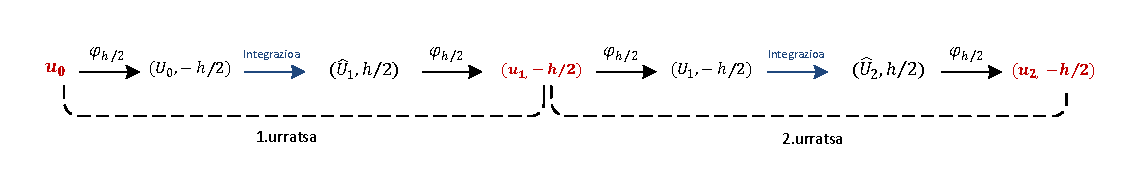
\includegraphics [width=16cm, height=4cm] {proiekzioa11}}
\caption{\small Metodoaren integrazio eskema orokorra. Metodoa simetrikoa eta sinplektikoa da.}
\label{fig:proiekzioa0}
\end{figure} 

Integrazioaren urrats guztietan ez baditugu emaitzak itzuli behar, bi urratsen arteko, $\varphi_{h/2}$ fluxuaren bi konputazioak, $\varphi_{h}$ fluxuaren konputazio bakarrarekin konputatuko dugu. Horretarako, proiekzio kontzeptua sortuko dugu (\ref{fig:proiekzioa2}~irudia).

\begin{figure} [h!]
\centerline{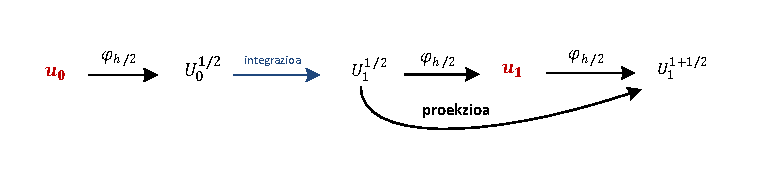
\includegraphics [width=14cm, height=4cm] {proiekzioa12}}
\caption{\small Proiekzioa: bi urratsen arteko, $\varphi_{h/2}$ fluxuaren bi konputazioak, $\varphi_{h}$ fluxuaren konputazio bakarrarekin konputatuko dugu}
\label{fig:proiekzioa2}
\end{figure} 


 Azkenik, emaitzak behar ditugun urratsetarako fluxua $\varphi_{-h/2}$ aplikatuko dugu (\ref{fig:proiekzioa1}~irudia). 

\begin{figure} [h!]
\centerline{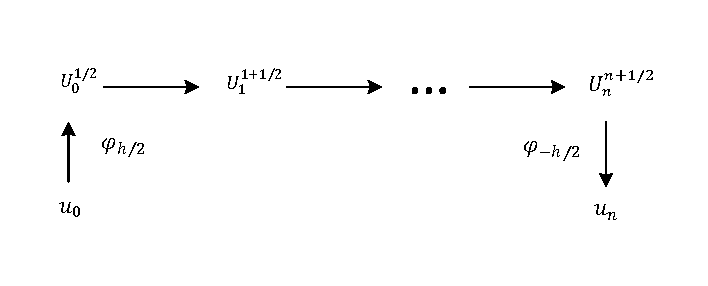
\includegraphics [width=14cm, height=5cm] {proiekzioa1}}
\caption{\small $u_i$ jatorrizko aldagaiak eta $U_i$ aldagai berriak adierazten dute. Lehenengo, $u_0$ jatorrizko aldagaien hasierako baliotik abiatuta, aldagai berriei dagokion $U_0^{1/2}$ hasierako balioa finkatuko dugu. Urrats bakoitza, integrazio eta proiekzioaren konposaketa da, \ref{fig:proiekzioa2}~irudian zehaztu dugun bezala. Erabiltzaileak definitutako urratsetarako, $u_n$ jatorrizko aldagaietan zenbakizko soluzioa itzuliko dugu}
\label{fig:proiekzioa1}
\end{figure} 


$u_i$ jatorrizko aldagaiak eta $U_i$ aldagai berriak adierazten duten notazioa erabiliko dugu. Hauek dira, integratzeko emango ditugun urratsak:
\begin{enumerate}
\item \emph{Startfun} funtzioa.

Lehenengo, $u_0$ jatorrizko aldagaien hasierako baliotik abiatuta, $\varphi_{h/2}$ fluxuaren konputazioaren bidez, aldagai berrietan dagokion hasierako balioa lortuko dugu.
\begin{align*}
u_0 \ \rightarrow \ U_0^{\frac{1}{2}}.
\end{align*}

\item \emph{Urratsa}.

Urratsa bi azpiurratsen konbinazio bezala ikusiko dugu: aldagai berriei Gaussen metodoaren bidezko integrazioaren urrats bat eta lortutako maitzei $\varphi_{h}$ bidez fluxuan $h$ aurrera egitea. Bigarren azpiurratsa fluxuaren bidez proiektatzea da. \ref{fig:proiekzioa2} irudian zehaztapenak eman ditugu. 
\begin{align*}
 U_0^{\frac{1}{2}} \ \rightarrow \ U_1^{\frac{1}{2}} \rightarrow \ U_1^{1+\frac{1}{2}}.
\end{align*}

Biribiltze errorea txikitzeko, proiekzioa doitasun altuan konputatzea garrantzitsua da. Modu honetan, batura konpensatua aplikatzerakoan zifra batzuk irabaziko ditugu. 

\item \emph{Outputfun} funtzioa.

Erabiltzaileak, $t$-ren balio jakin batzuetan $u(t)$ balioen zenbakizko soluzioak nahiko ditu, kasu horietan $\varphi_{-h/2}$ fluxuaren konputazioaren bidez, $U_i^{i+\frac{1}{2}}$ balioetatik $u_i$ jatorrizko aldagaien balioak lortuko dira:
\begin{align*}
U_n^{n+\frac{1}{2}} \ \rightarrow \ u_n.
\end{align*}


\end{enumerate}


Gauss metodoa, neurri batean  Splitting eta konposizio metodoen baliokideak dira. 
\begin{align*}
\text{Konposizio metodoa} \ \ &\equiv \ \ \text{Gauss metodoa aldagai aldaketa gabe}.\\
\text{Splitting metodoa} \ \ &\equiv \ \  \text{Gauss metodoa aldagai aldaketarekin}.
\end{align*}

Splitting metodoekiko antzekotasuna azaltzeko, (\ref{eq:stverlet})~\emph{Störmer-Verlet} Splitting metodoarekin konparatuko dugu. \emph{Störmer-Verlet} metodoa, era honetan aplikatzen da: $h/2$ fluxua aplikatu, perturbazioak kalkulatu eta berriz  $h/2$ fluxua aplikatu. Fluxuaren aldagai aldaketarekin, gauza bera egiten ari gara: $h/2$ fluxua aurreratu, perturbazioak kalkulatu (aldagai berrietan eta beraz, hobeto kalkulatzen dugu), $h/2$ fluxua aurreratu. 


\section{Zenbakizko esperimentuak.}
\label{s:7espmt}

Zenbakizko esperimentuetarako, puntu-finkoaren iterazioan oinarritutako Gauss metodoaren inplementazioa (\ref{chap:IRK-PF}~kapitulua) erabili dugu eta eguzki-sistemaren ekuazio diferentzialei, Kepler-en fluxuan oinarritutako aldagai aldaketa aplikatu diegu. $s=6,8,9,16$ ataletako Gauss metodoak exekutatu ditugu eta metodo eraginkorrena aukeratu dugu, \emph{CO1035} konposizio eta \emph{ABAH1064} Splitting  metodoekin konparatzeko.

Esperimentu hauen konputaziorako, $64$-biteko (bikoitza) eta $80$-biteko (\emph{long double}) doitasunak nahasi ditugu. Konputazioaren zati nagusiena, $64$-biteko doitasunean egin dugu eta proiekzioa kalkulatzeko, $80$-biteko doitasuna aplikatu dugu. Era honetan, modu merkean soluzioaren doitasuna hobetzea lortu dugu.

Gauss metodoaren exekuzio sekuentziala eta paraleloak egin ditugu. $s$ atalen funtzioen balioztapena, 
\begin{align*}
F_{n,i}=f(Y_{n,i}), \ i=1,\dots,s,
\end{align*}      
independenteak dira eta paraleloan kalkula daitezke. Exekuzio paraleloak $s=8$ metodoarentzat egin ditugu, eta bi kasu aztertu ditugu: hari kopuruak $2$ eta $4$. 

\subsection{Problemak.}


9-planeten problema (\ref{sss:9body}~atala) erabili dugu integrazioetarako. Hasierako balioak \emph{DE-430} efemerideen artikulutik hartu ditugu: planeten masak  \ref{tab:9bodymas}~taulan laburtu ditugu; eta hasierako kokapen eta abiadurak \ref{tab:9bodyhas}~taulan aurki daitezke.

Koordenatu heliozentrikoei dagokien  Hamiltondar sistema (\ref{eq:nbodyHel}),
\begin{align*}
&H(q,p)=H_K(q,p)+H_I(q,p),
%&H(q,p)=\sum\limits_{i=1}^{N}\bigg(\frac{\|P_i\|^2}{2 \mu_i} -\frac{G m_0 m_i}{\|Q_i\|}\bigg)+H_I(q,p)
\end{align*}
integratu dugu. $H_K(q,p)$ mugimendu Kepleriarrari dagokion Hamiltondarraren aldea da  eta $H_I(q,p)$, perturbazioei dagokien Hamiltondarraren aldea da. 
%Kepler-en fluxuan oinarritutako aldagai aldaketaren bidez, alde Kepleriarra ekuazioetatik desagerrarazten dugu.    

Integrazioen tartea, $t_{end}=10^6$ egunetakoa da eta zenbakizko integrazioetan, $h$-ren balio ezberdinak erabili ditugu. $s=6$ metodoarentzat urrats luzerak aukeratu ditugu eta gainontzeko metodoentzat, $s$-atalen araberako urrats luzera proportzionalak finkatu ditugu:
\begin{align*}
&s=6: \quad  \ \ h=2^{k/4}, \ k=4,\dots,28, \\
&s=8: \quad  \ \ (8/6)h, \\
&s=9: \quad  \ \ (9/6)h, \\
&s=16: \quad (16/6)h. \\
\end{align*} 

Zenbakizko esperimentuetarako, aldagai aldaketa planeta guziei aplikatzea erabaki dugu. $9$-planeten probleman, gorputz kopurua txikia denez,  Kepler fluxuaren gainkarga esanguratsua da eta  barne-planetei bakarrik aplikatzea, eraginkorragoa izan daiteke. Baina, gorputz gehiago kontsideratzen baditugu (esaterako ilargia eta asteroide nagusienak) edo eguzki-sistemaren eredu konplexuagoetan (esaterako erlatibitate efektua gehitzerakoan), perturbazio aldearen konputazioa nagusituko da eta Kepler fluxuaren kalkuluak pisua galduko luke. 


\subsection*{Lehen esperimentua.}


\ref{fig:esp81s}~irudian, $s=6,8,9,16$ ataletako metodoen eraginkortasun grafikoak irudikatu ditugu. Eraginkortasuna, energia errore erlatibo maximoaren arabera neurtu dugu: lehen kasuan, \emph{CPU}-denborarekiko (exekuzio paraleloetan \emph{Wall time}) eta bigarren kasuan, ekuazio diferentzialen ebaluazio kopuruarekiko (\emph{FCN}). Eraginkortasuna \emph{CPU}-rekiko, problema zehatz honetarako gertatzen dena azaltzen digu eta eraginkortasuna \emph{FCN}-rekiko, metodoak problema erreal batean nola jokatuko luke erakusten digu. 


\begin{figure}[h!]
\centering
\begin{tabular}{c c}
\subfloat[ Exekuzioa sekuentziala: CPU Time.]
{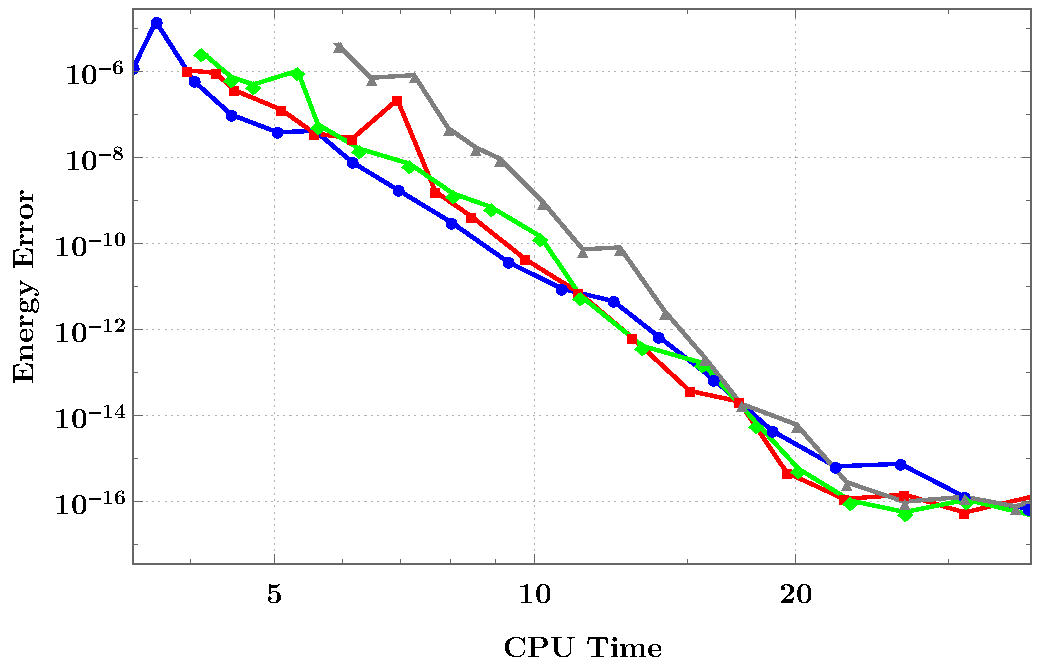
\includegraphics[width=.5\textwidth]{esperimentua811}}
&
\subfloat[ Exekuzioa sekuentziala: FCN.]
{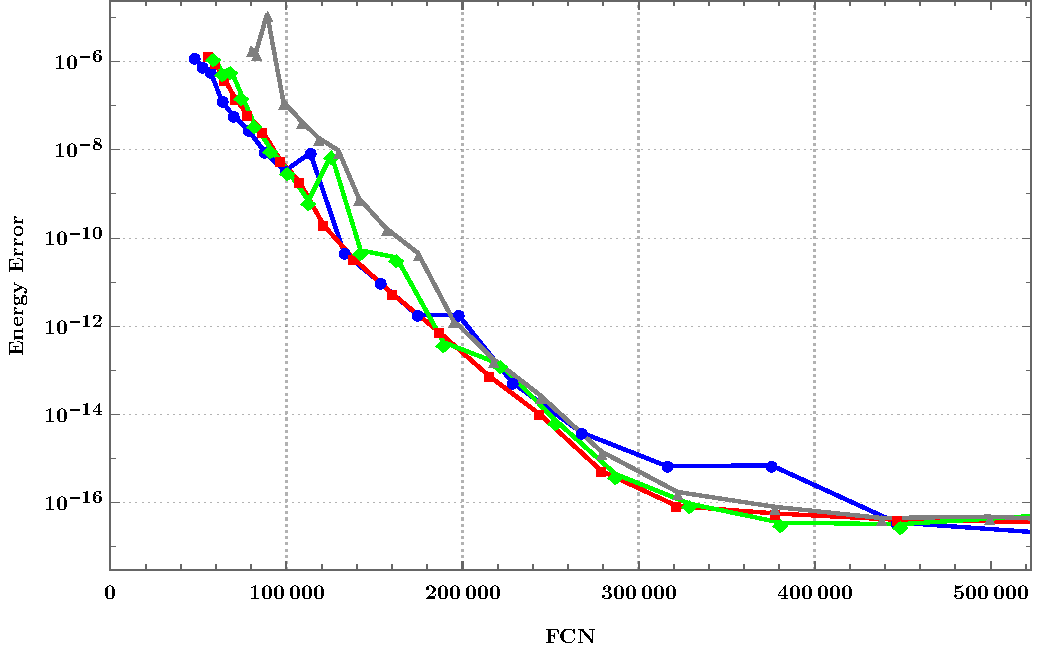
\includegraphics[width=.5\textwidth]{esperimentua812}}\\
\subfloat[Exekuzio paraleloa (hariak=$2$):Wall Time.]
{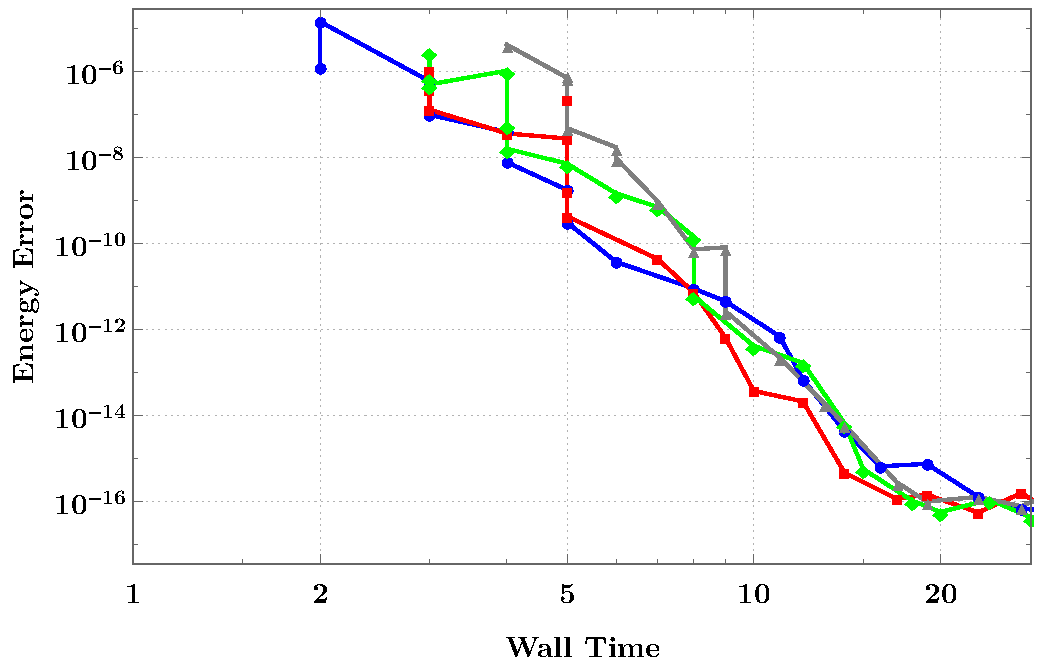
\includegraphics[width=.5\textwidth]{esperimentua813}}
&
\subfloat[Exekuzio paraleloa (hariak=$4$): Wall Time.]
{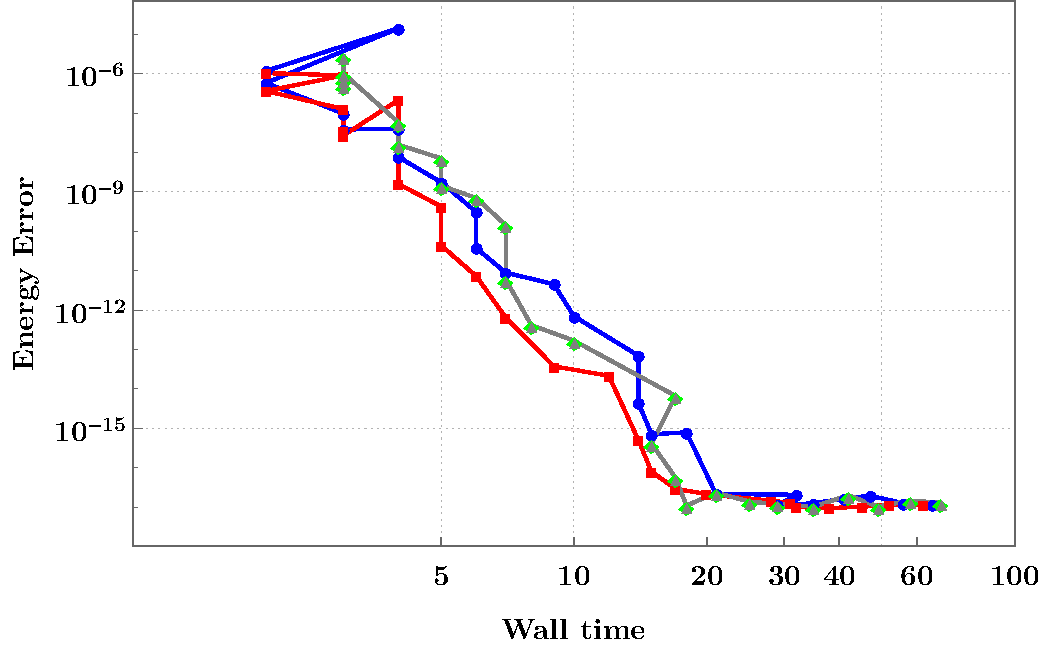
\includegraphics[width=.5\textwidth]{esperimentua814}}
\end{tabular}
\caption{\small 
Eraginkortasun grafikoak eskala logaritmiko bikoitzean irudikatu ditugu. Batetik, ardatz bertikalean, energiaren errore erlatibo maximoa eman dugu. Bestetik, ardatz horizontalean, (a),(c),(d) irudietan CPU denbora (exekuzio paralelotan Wall-Time) eta (b) irudian, ekuazio diferentzialen ebaluazio kopurua (FCN) erakutsi dugu. (a)  konputazioa modu sekuentzialean egin dugu. (c) eta (d) modu paraleloan:  (c) kasuaren exekuzioa hari kopurua $2$ da eta (d) kasuan hari kopurua $4$ izan dira. Irudi bakoitzean, Gauss metodoaren $s$ ataletako lau integrazio konparatu ditugu: $s=6$  urdinez, $s=8$ gorriz, $s=9$ berdez, eta $s=16$ grisez. }
\label{fig:esp81s}
\end{figure}

Exekuzio sekuentzialak eta exekuzio paraleloak aztertuz,  Gauss metodo eraginkorrena aukeratu nahi dugu. Horretarako, biribiltze errorea nagusitzen hasten den inguruko unean gertatutakoa aztertu dugu: $s=8,9,16$ metodoak, $s=6$ metodoa baino eraginkorragoak azaldu zaizkigu. $s=8,9,16$ metodoak beraien artean oso antzekoak izanik, $s=8$ ataleko Gauss metodoa aukeratu dugu. Bestalde, exekuzio paraleloa, sekuentziala baino eraginkorragoa da eta $4$ hari erabili dugun integrazioa, eraginkorrena azaldu zaigu.  

\subsection*{Bigarren esperimentua.}


%$s=8$ metodoarentzat, birbiltze errorea hasten den uneko urrats luzera hartu dut: $k=12, \ h=10,667$. Kokapen errore erlatiboaren estimazioa, $h/2$ integrazioarekiko diferentzia gisa kalkulatu ditugu.


\subsubsection*{Energiaren eboluzioa}


\ref{fig:esp83}~irudian energiaren errore erlatiboaren eboluzioa erakutsi dugu lau integrazio metodo hauetarako:
\begin{enumerate}
\item Gauss metodoa $s=8$ (proiekzioa \emph{long double} doitasunarekin). Integraziorako $h=10.63$ urrats luzera erabili dugu.
\item Gauss metodoa $s=8$ (proiekzioa \emph{double} doitasunarekin). Integraziorako $h=10.63$ urrats luzera erabili dugu.
\item \emph{ABAH1064} Splitting metodoa. Integraziorako $h=4.76$ urrats luzera erabili dugu.
\item \epmh(CO1035) Konposizio metodoa. Integraziorako $h=4.76$ urrats luzera erabili dugu.
\end{enumerate}

\begin{figure}[h!]
\centering
\begin{tabular}{c c}
\subfloat[Gauss metodoa ($s=8$).]
{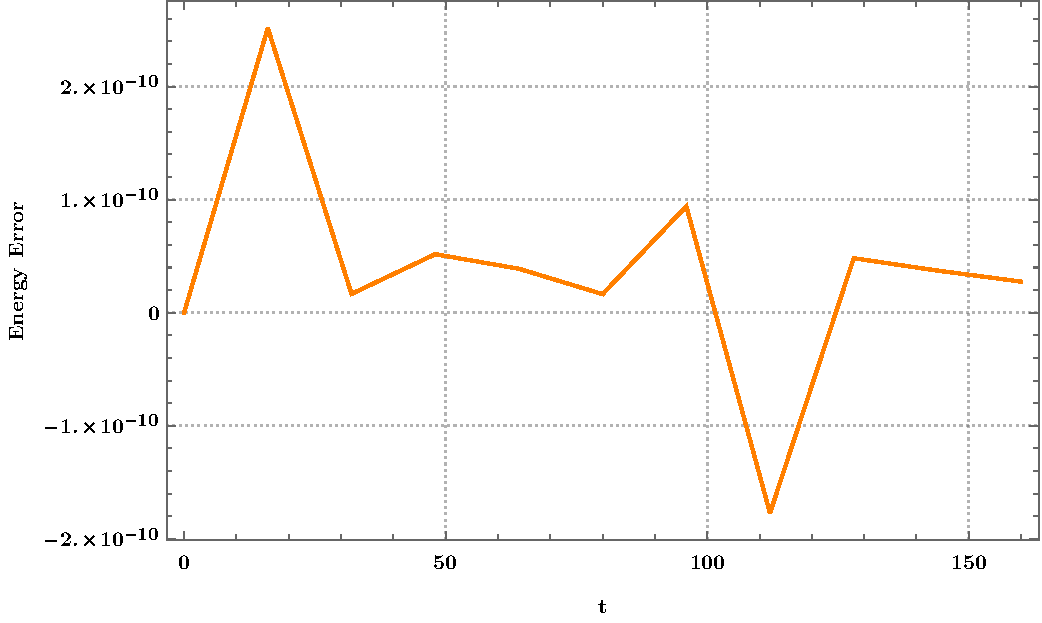
\includegraphics[width=.5\textwidth]{esperimentua831}}
&
\subfloat[ABAH1064 eta CO1035]
{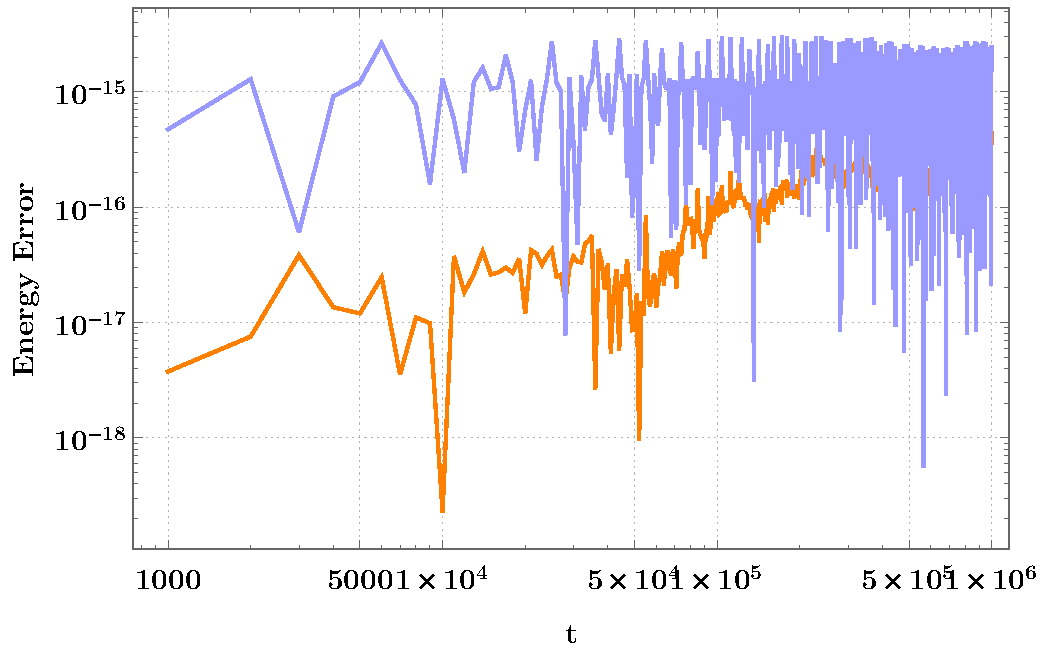
\includegraphics[width=.5\textwidth]{esperimentua832}}
\end{tabular}
\caption{\small Energia errorearen eboluzioa lau integrazio metodoetarako erakutsi dugu. Ezkerreko irudian, $s=8$ ataletako Gauss metodoaren $h=10,667$ urrats luzerarekin egindako integrazioak erakutsi ditugu: proiekzioa \emph{long double} doitasunarekin (laranjaz) eta proiekzioa \emph{double} doitasunarekin (urdinez). Eskuineko irudian, Splitting/Konposizio metodoak erakutsi ditugu: ABAH1064 (laranjaz) eta CO1035(urdinez)}
\label{fig:esp83}
\end{figure}


\subsubsection*{Kokapen eta abiadura errore estimazioak}


\ref{fig:esp84}~irudian, Gauss ($s=8$) eta \emph{ABAH1064} metodoentzako, kokapen eta abiaduraren erroreen estimazioak erakutsi ditugu. Erroreak estimatzeko, urrats txikiagoako integrazioaren soluzioarekiko diferentzia gisa kalkulatu dugu. 
Gauss metodoaren integrazioan, urrats luzera handiago erabili arren, barne-planeten kokapen eta abiaduren errore estimazioak txikiagoak izan dira. 

\begin{figure}[h!]
\centering
\begin{tabular}{c c}
\subfloat[Gauss metodoa (kokapen errorea)]
{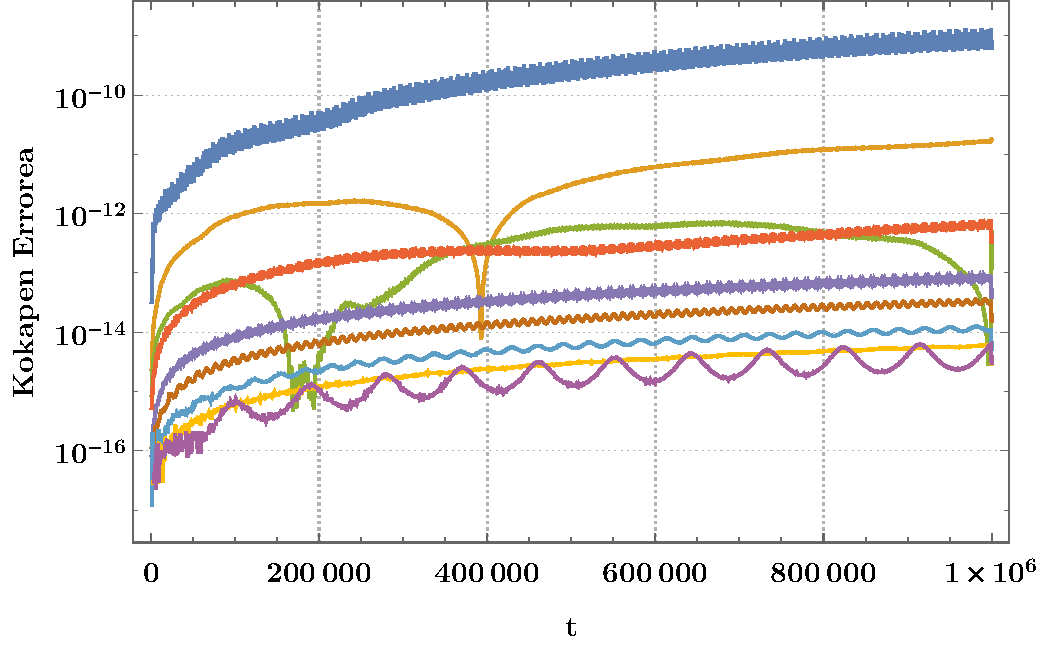
\includegraphics[width=.5\textwidth]{esperimentua841}}
&
\subfloat[Gauss metodoa (abiadura errorea)]
{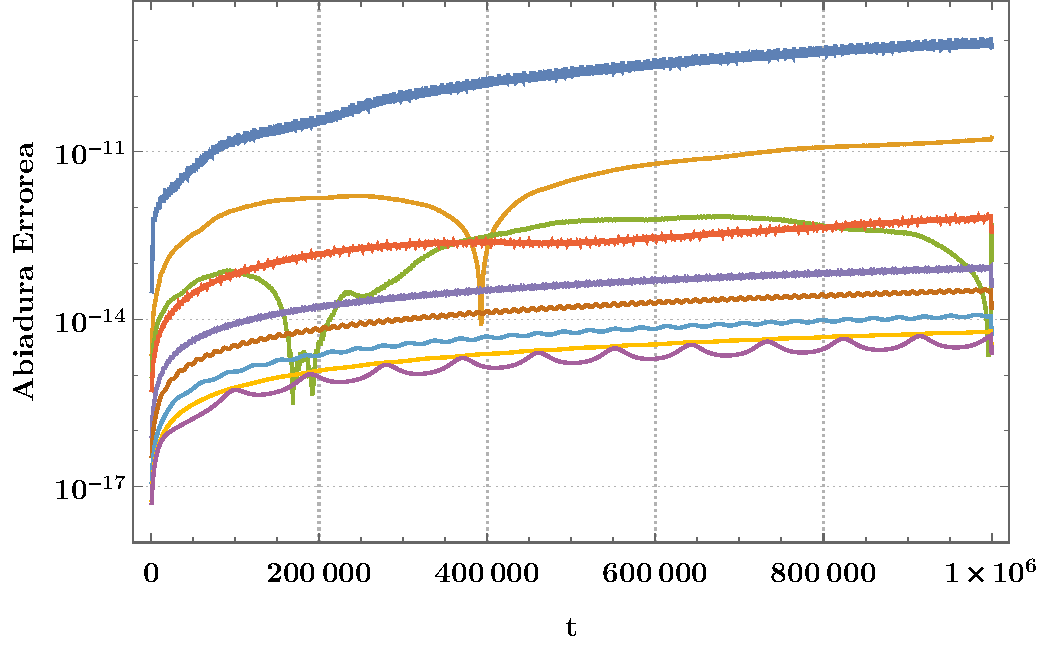
\includegraphics[width=.5\textwidth]{esperimentua842}}
\\
\subfloat[ABAH1064 (Kokapen errorea)]
{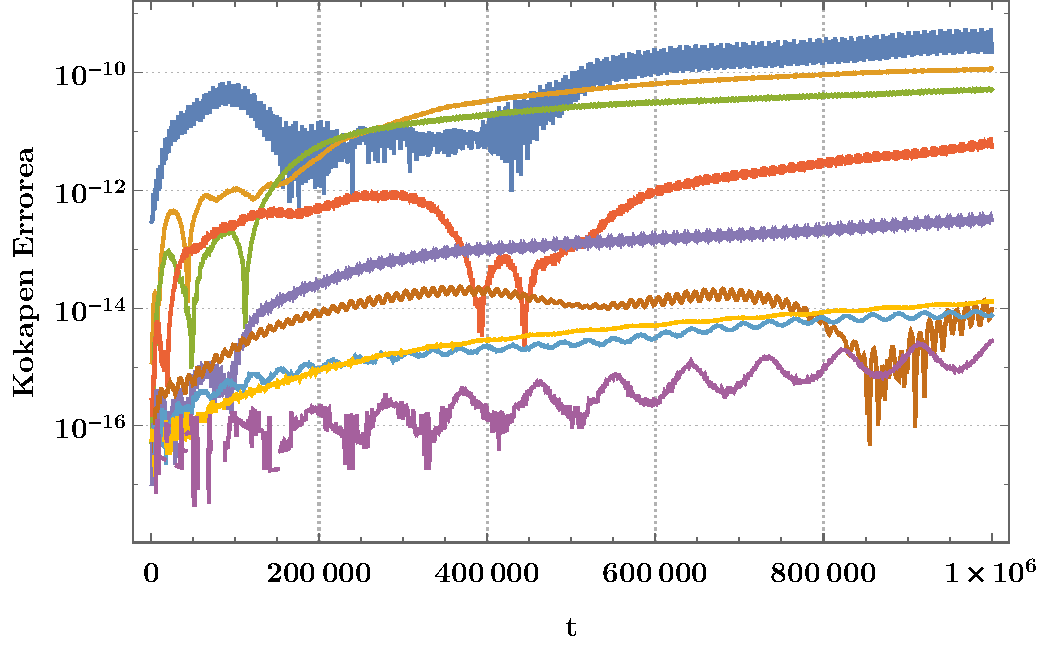
\includegraphics[width=.5\textwidth]{esperimentua843}}
&
\subfloat[ABAH1064 (Abiadura errorea)]
{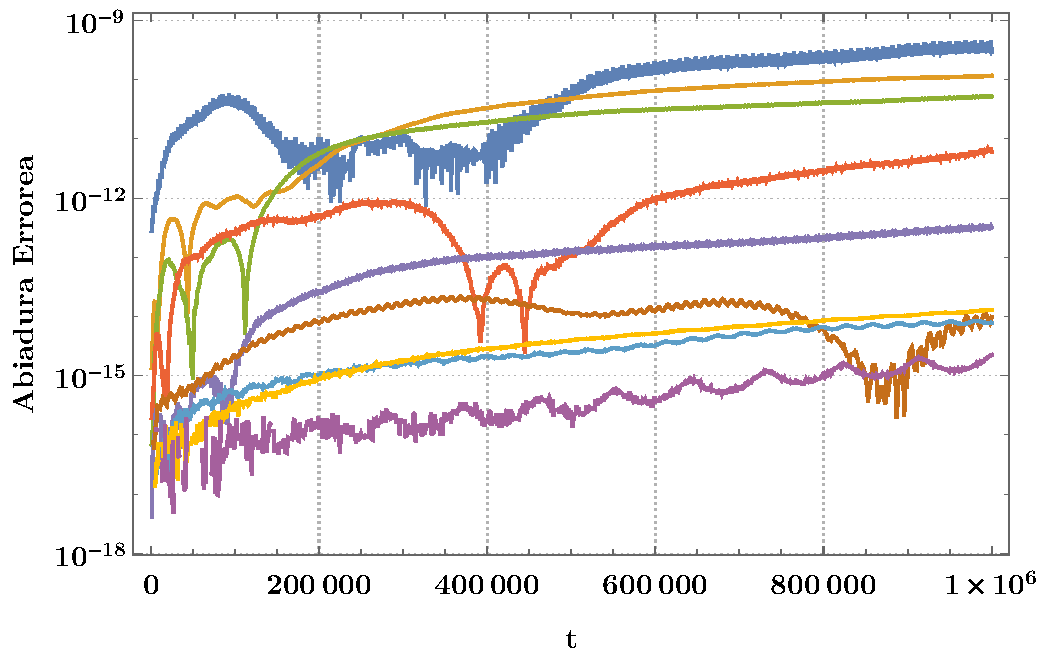
\includegraphics[width=.5\textwidth]{esperimentua844}}
\end{tabular}
\caption{\small Kokapen eta abiaduraren erroreen estimazioak erakutsi ditugu. (a) eta (b) irudietan, $s=8$ ataletako Gauss metodoaren errore estimazioak eman ditugu, $h=10,667$ urrats luzerarekin integratuz. (c) eta (d) irudietan, \emph{ABAH1064} Splitting metodoaren errore estimazioak eman ditugu, $h=4.76$ urrats luzerarekin integratuz. Kolore bakoitza planeta bakoitzari dagokion errorea da: Merkurio (urdin ilunez), Artizarra (marroi argiz), Lurra (berdez), Marte (gorriz), Jupiter (more argiz), Saturno (marroi ilunez), Urano (urdin argiz), Neptuno (laranja argiz), Pluto (morez)}
\label{fig:esp84}
\end{figure}

\textcolor{red}{irudi berriak !!!!!}
\begin{figure}[h!]
\centering
\begin{tabular}{c c}
\subfloat[Gauss metodoa (kokapen errorea)]
{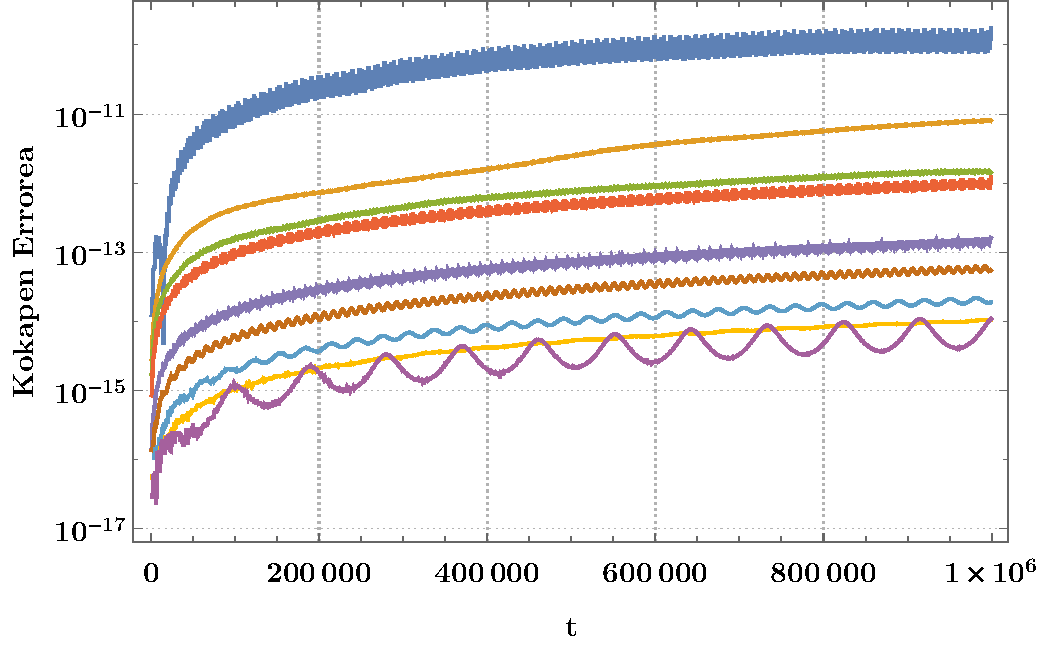
\includegraphics[width=.5\textwidth]{esperimentua8410}}
&
\subfloat[Gauss metodoa (abiadura errorea)]
{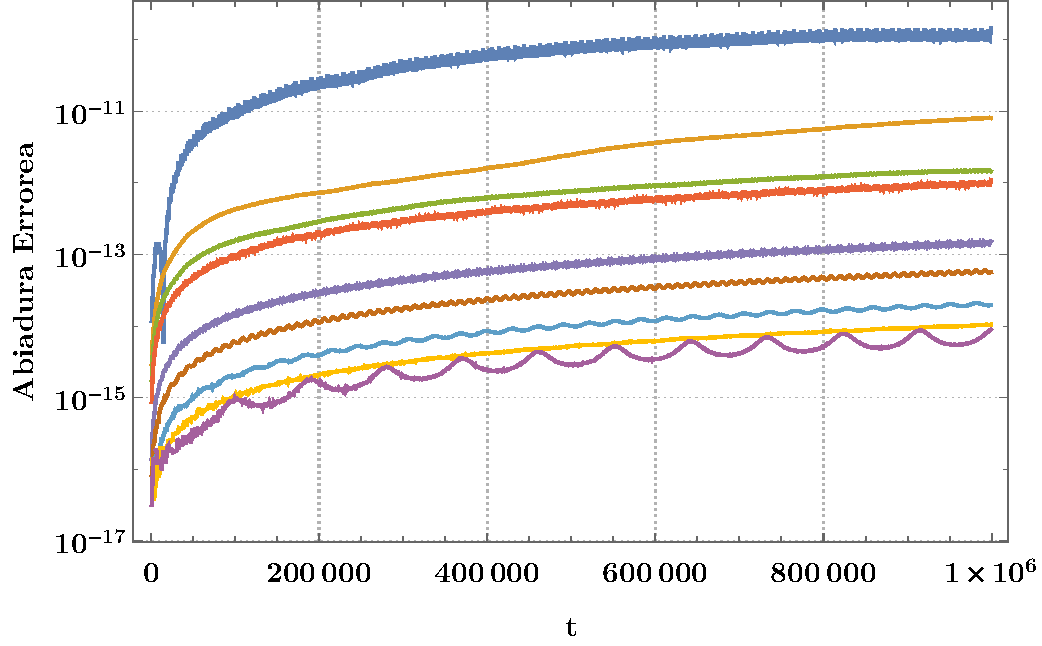
\includegraphics[width=.5\textwidth]{esperimentua8420}}
\\
\subfloat[ABAH1064 (Kokapen errorea)]
{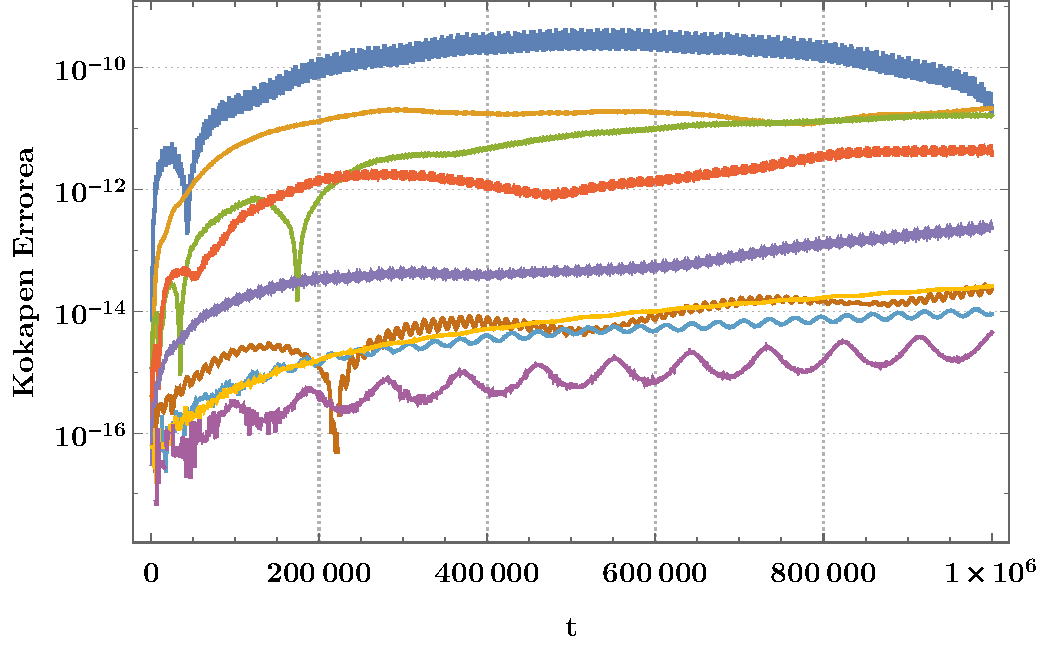
\includegraphics[width=.5\textwidth]{esperimentua8430}}
&
\subfloat[ABAH1064 (Abiadura errorea)]
{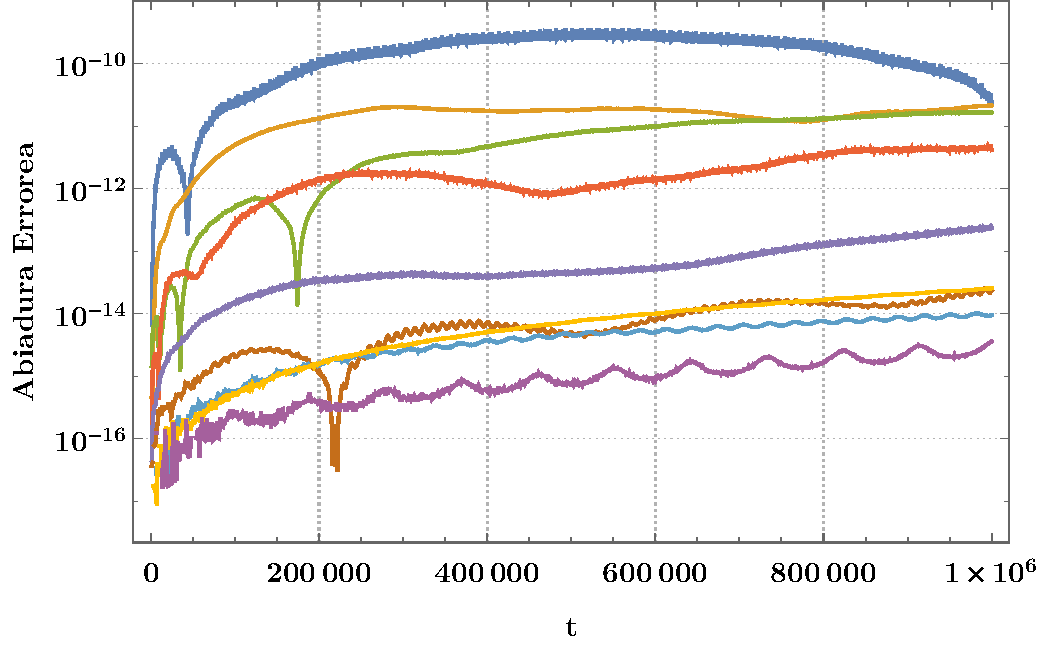
\includegraphics[width=.5\textwidth]{esperimentua8440}}
\end{tabular}
\caption{\small Kokapen eta abiaduraren erroreen estimazioak erakutsi ditugu. (a) eta (b) irudietan, $s=8$ ataletako Gauss metodoaren errore estimazioak eman ditugu, $h=4,48$ urrats luzerarekin integratuz. (c) eta (d) irudietan, \emph{ABAH1064} Splitting metodoaren errore estimazioak eman ditugu, $h=2.38$ urrats luzerarekin integratuz. Kolore bakoitza planeta bakoitzari dagokion errorea da: Merkurio (urdin ilunez), Artizarra (marroi argiz), Lurra (berdez), Marte (gorriz), Jupiter (more argiz), Saturno (marroi ilunez), Urano (urdin argiz), Neptuno (laranja argiz), Pluto (morez)}
\label{fig:esp84B}
\end{figure}



\subsection*{Hirugarren esperimentua.}


Hirugarren esperimentu honetan, biribiltze errorearen azterketa egin dugu eta horretarako, momentu angeluarraren errore erlatiboaren eboluzioa eman dugu. Momentu angeluarraren trunkatze errorea beti zero da, metodo sinplektikoek inbariante koadratikoak zehazki mantentzen dituzte. \ref{fig:esp85}~irudian, Gaussen $s=8$ ataletako metodoarekin, $h=9.0$ eta $h=10.63$ urrats luzerarekin integrazioen soluzioen momentu angeluarraren errorea erakutsi dugu.  


\begin{figure}[h!]
\centering
\begin{tabular}{c c}
\subfloat[Momentu angeluarra $h=9.0$.]
{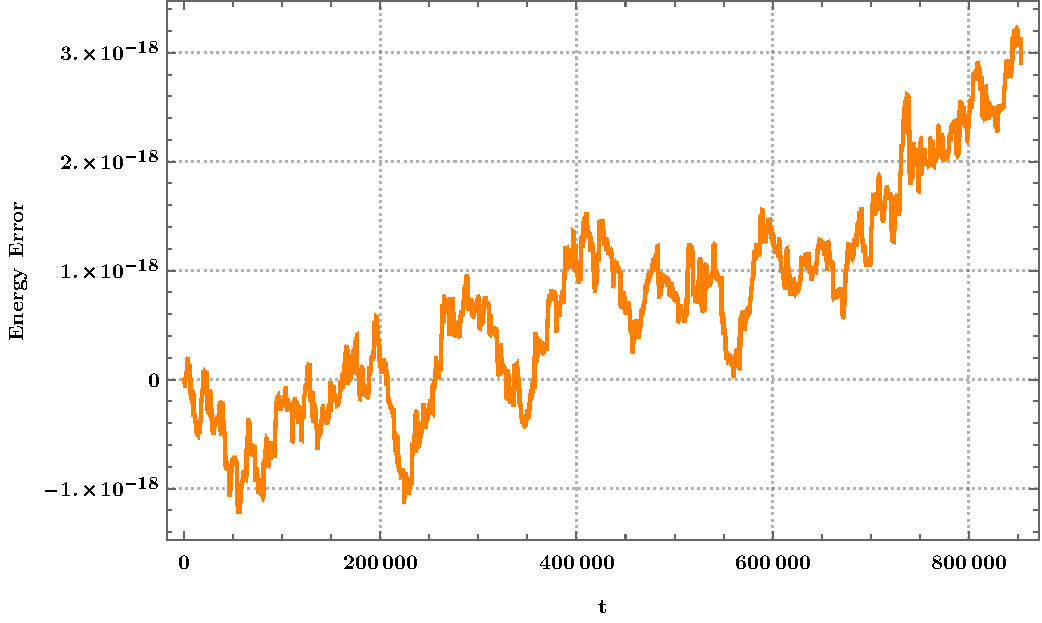
\includegraphics[width=.5\textwidth]{esperimentua851}}
&
\subfloat[Momentu angeluarra $h=10.63$]
{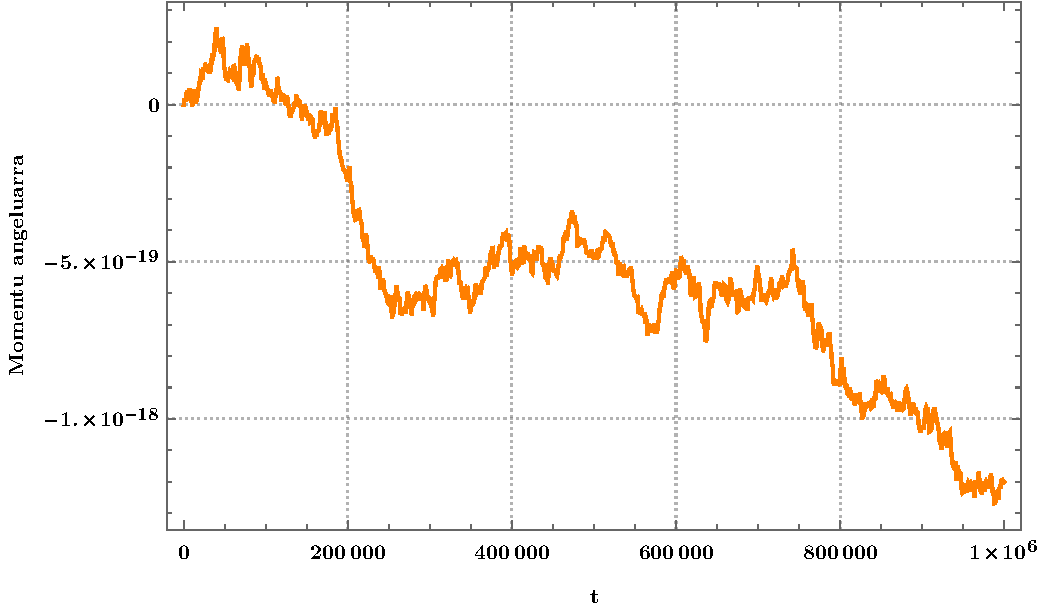
\includegraphics[width=.5\textwidth]{esperimentua852}}
\end{tabular}
\caption{\small Momentu angeluarraren errore erlatiboaren eboluzioa erakutsi dugu. Gaussen $s=8$ ataletako metodoa integratu dugu $h=9.0$ eta $h=10.63$ urrats luzerarekin. }
\label{fig:esp85}
\end{figure}



\subsection*{Laugarren esperimentua.}


\ref{fig:esp82}~irudian, Gauss metodoa eta konposizio/Splitting metodoen arteko eraginkortasunaren konparaketa egin dugu. $s=8$ ataletako Gauss metodoa, modu sekuentzialean eta modu paraleloan exekutatu dugu. Esperimentu hauetan, eguzki-sistemaren eredu sinplearen integraziorako, Splitting metodoak oso eraginkorrak azaldu zaizkigu. Gauss metodoaren exekuzioa paralelizatzeak abantaila erakusten du baina hala ere, Splitting metodoak eraginkorragoak dira.

Dena den, eredu errealistagoak (gorputz kopurua handitzen delako edota erlatibitate efektua kontutan hartzen delako) integratzeko, Gauss metodoak eraginkorragoak bilakatzea espero da. Splitting metodoen konputazioak, modu trinkoan kalkulatu behar dira, hau da, atalen konputazioak sekuentzialki exekutatzen dira eta  ez ditu aldaerak onartzen. Gauss metodoaren ekuazio inplizituak ebazteko, ordea, teknika ezberdinak konbina daitezke eta eraginkortasuna hobetzeko aukera asko eskaintzen dizkigu. Adibidez, iterazio gehienak problemaren eredu sinple batekin, doitasun baxuan kalkula daitezke  \cite{Beylkin2014} eta bukaerako iterazio pare bat eredu osoarekin, doitasun altuan. Gauss metodoaren $s$-ataletako funtzioen ebaluazioak  modu paraleloan exekutatu daitezke eta eguzki-sistemaren eredu konplexuagoa kontutan hartzen den neurrian, paralelizazioak abantaila handiagoa suposatuko du.

\begin{figure}[h!]
\centering
\begin{tabular}{c c}
\subfloat[Exekuzio sekuentziala: CPU Time.]
{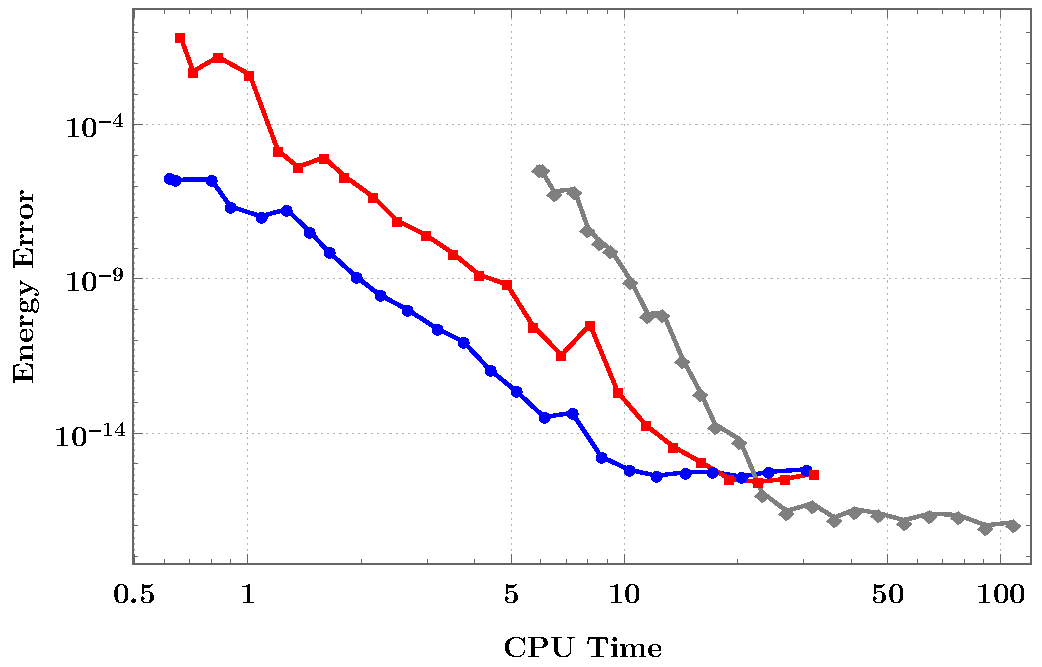
\includegraphics[width=.5\textwidth]{esperimentua821}}
&
\subfloat[Exekuzio sekuentziala: FCN.]
{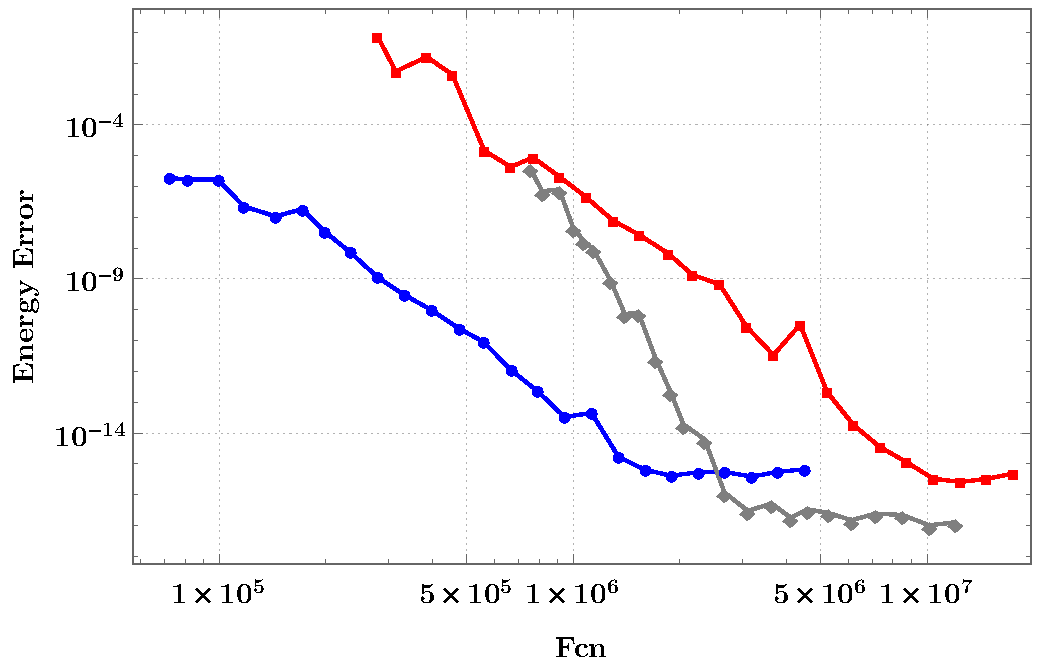
\includegraphics[width=.5\textwidth]{esperimentua822}}\\
\subfloat[Exekuzio paraleloa (hariak=$2$) Wall Time.]
{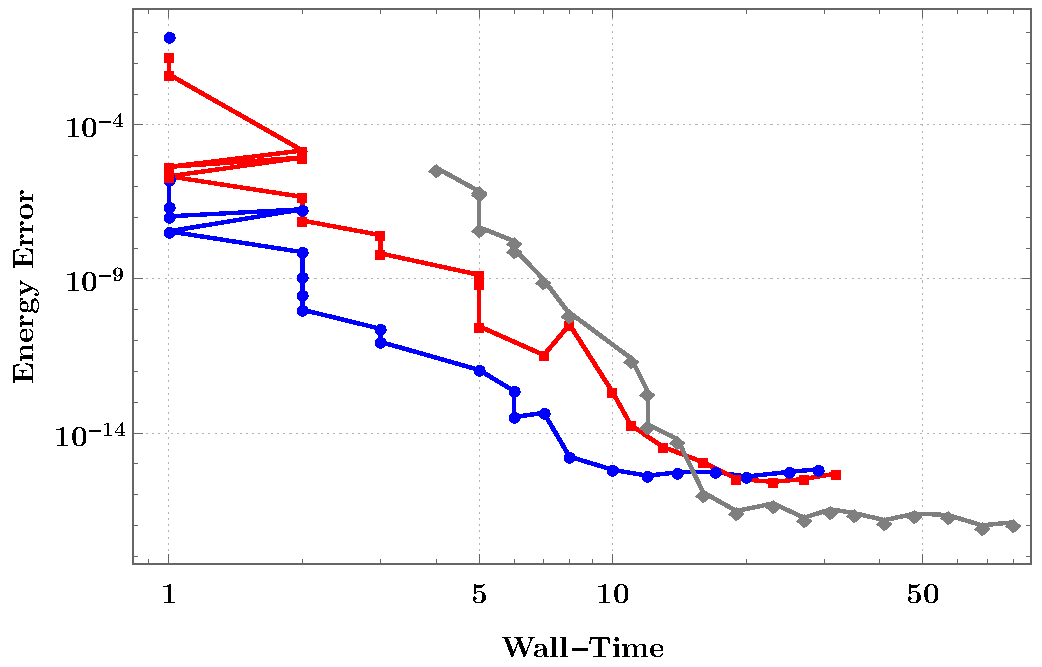
\includegraphics[width=.5\textwidth]{esperimentua823}}
&
\subfloat[Exekuzio paraleloa (hariak=$4$) Wall Time.]
{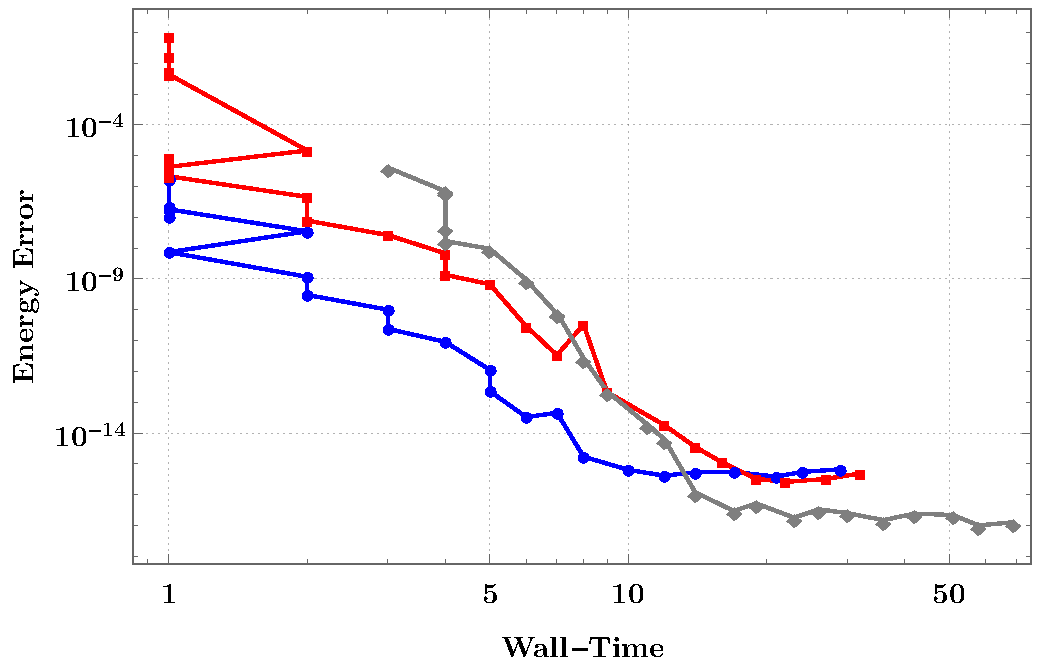
\includegraphics[width=.5\textwidth]{esperimentua824}}
\end{tabular}
\caption{\small 
Eraginkortasun grafikoak eskala logaritmiko bikoitzean irudikatu ditugu. Batetik, ardatz bertikalean, energiaren errore erlatibo maximoa eman dugu. Bestetik, ardatz horizontalean, (a),(c),(d) irudietan CPU denbora (exekuzio paralelotan Wall-Time) eta (b) irudian, ekuazio diferentzialen ebaluazio kopurua (FCN) erakutsi dugu. (a) konputazioa modu sekuentzialean egin dugu. (c) eta (d) modu paraleloan:  (c) kasuaren exekuzioa hari kopurua $2$ da eta (d) kasuan hari kopurua $4$ izan dira. Irudi bakoitzean,  hiru integrazio metodo konparatu ditugu: $s=6$ Gauss metodoa grisez, $ABAH1064$  urdinez eta $CO1035$ gorriz
}
\label{fig:esp82}
\end{figure}

%\begin{figure}[h!]
%\centering
%\begin{tabular}{c c}
%\subfloat[$s=16$ Exekuzio sekuentziala: CPU-denbora.]
%{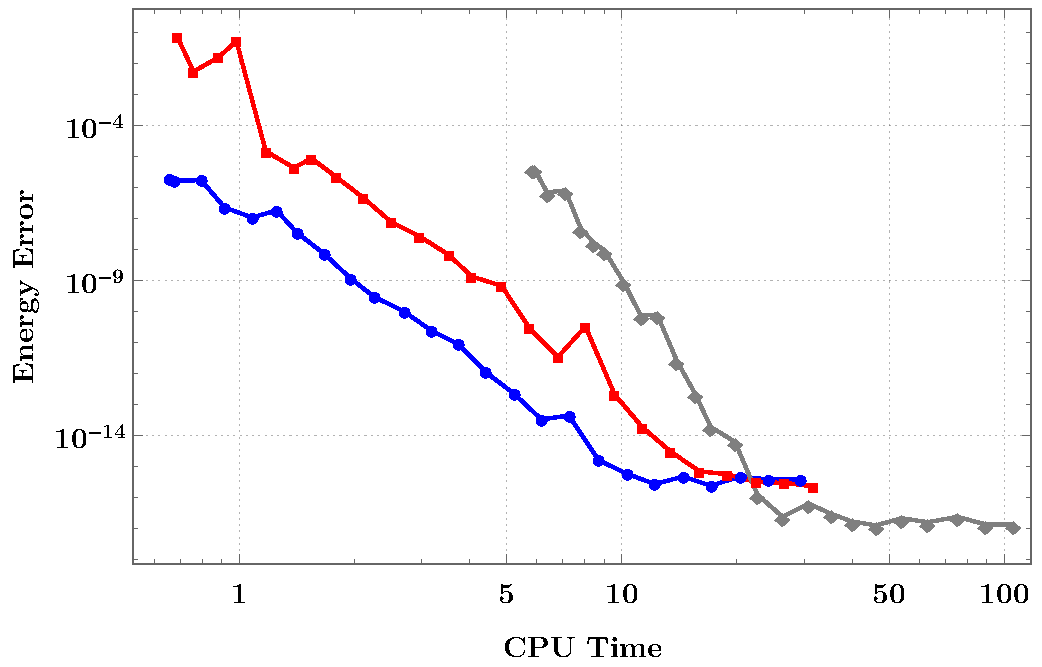
\includegraphics[width=.5\textwidth]{esperimentua861}}
%&
%\subfloat[$s=16$ Exekuzio sekuentziala:: FCN.]
%{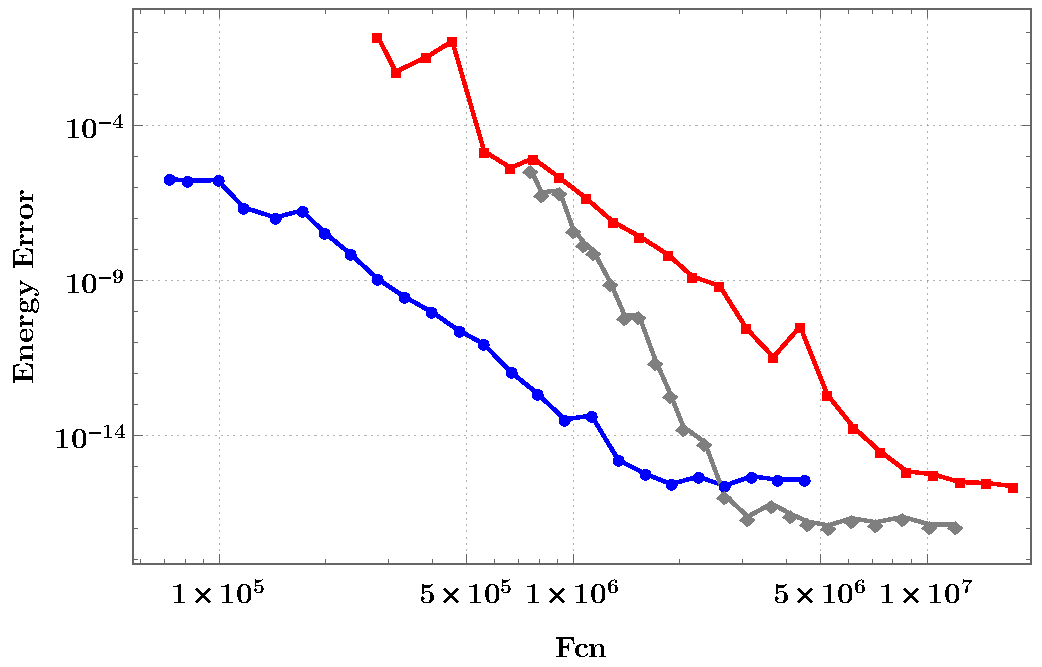
\includegraphics[width=.5\textwidth]{esperimentua862}}\\
%\subfloat[$s=16$ Exekuzio paraleloa: hariak=$2$.]
%{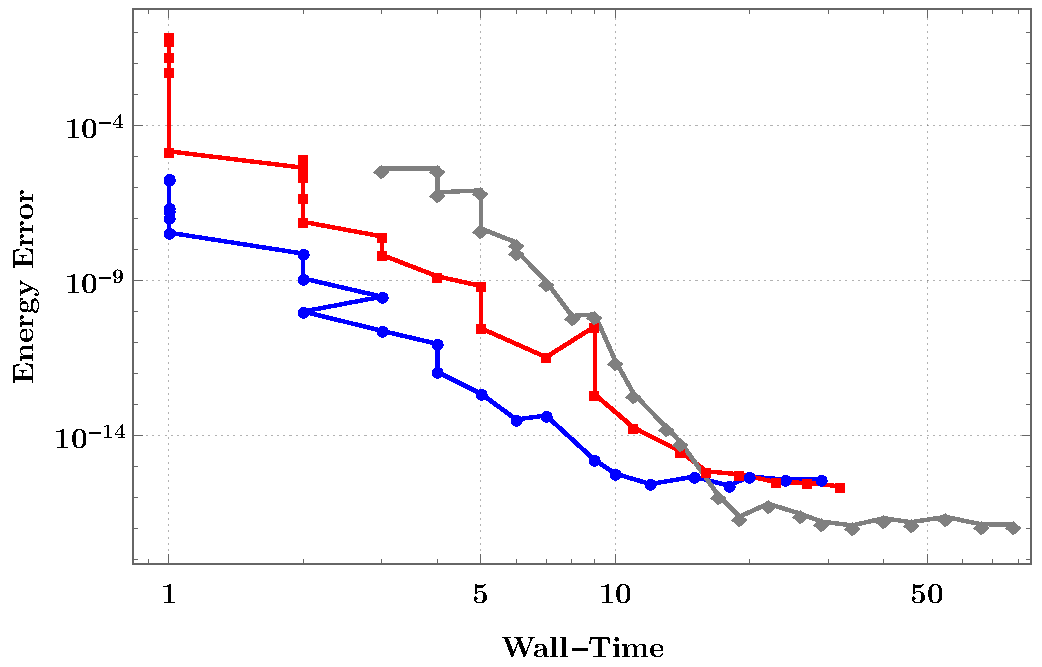
\includegraphics[width=.5\textwidth]{esperimentua863}}
%&
%\subfloat[$s=16$ Exekuzio paraleloa: hariak=$4$.]
%{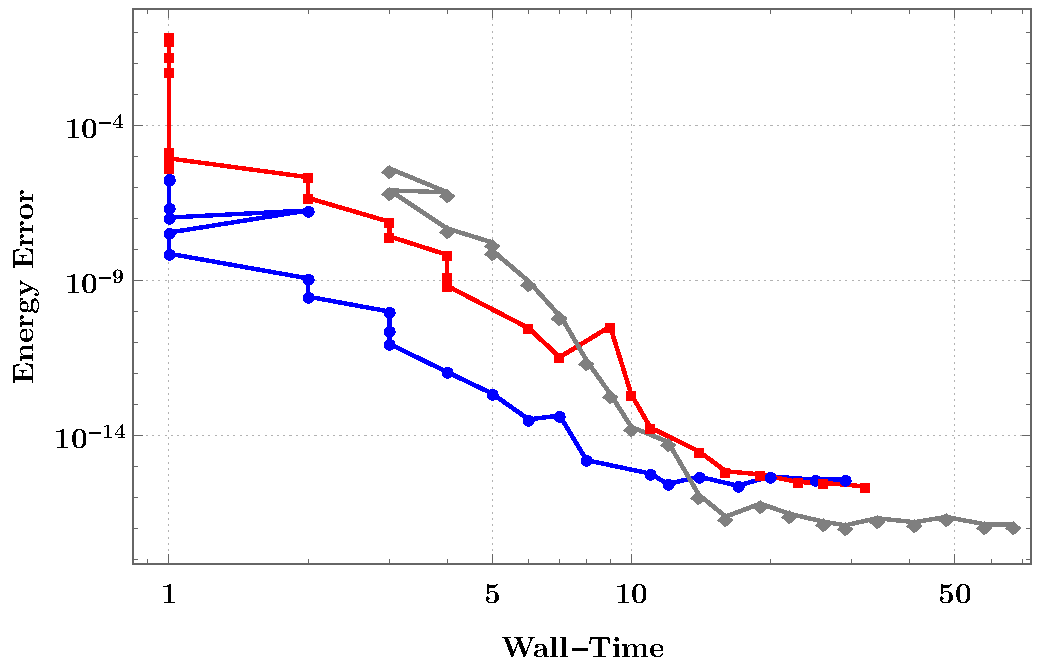
\includegraphics[width=.5\textwidth]{esperimentua864}}
%\end{tabular}
%\caption{\small 
%Eraginkortasun grafikoak irudikatu ditugu: ezkerrean energiaren errore maximoa, CPU denborarekiko; eskuinean ekuazio diferentzialen ebaluazio kopuruarekiko (FCN). Lau integrazio metodo konparatu ditugu: $ABAH1064$  urdinez, $CO1035$ gorriz,  eta \emph{IRKFLUXU} grisez}
%\label{fig:esp82}
%\end{figure}


\section{Laburpena.}